\section{Introduction}
\label{sec:intro}

A growing share of language-model calls in production software ask for a decision rather than a
paragraph: which of forty queues a ticket belongs in, whether a transaction is fraud, how severe an
alert is, which tool an agent should call next. The caller needs a probability distribution over a
label set it defines at request time, and it needs to know when none of the labels fit. The usual
route to that distribution goes through text. The model generates an answer symbol or a JSON object,
or the caller constrains decoding, or it compares candidate log-probabilities. Each of these inherits
the costs of the generative interface: decoding latency, parsing, and a well-documented sensitivity to
how the answer is written, including option-order and option-symbol biases
\citep{zheng2024selectionbias,pezeshkpour2024optionorder} and first-token probabilities that disagree
with the text the model goes on to produce \citep{wang2024firsttoken}.

A pretrained model does not need to write its answer down for the decision to exist. When a causal
language model reads a question followed by a list of options, the winning option is already decodable
from its hidden states before the answer symbol is bound \citep{wong2026models}. \textbf{Typical}
makes that internal decision the deployed interface. A call has the signature
\[
  (\text{state},\ \text{typed question},\ \text{runtime candidate set}) \;\longmapsto\;
  \big(P(\cand{1}),\dots,P(\cand{\numcands}),\ \pnull\big),
\]
and nothing is generated or parsed. The state (a ticket, a policy document, an agent trace) is encoded
once into a key-value cache. Each question against it is a short causal suffix containing the question
and its candidates, and a head at 71\% of the backbone's depth reads the terminal decision state against
each candidate's own contextual hidden state. The output type is a contract on the returned
distribution: categorical \emph{Choice}, ordinal \emph{Score}, Bernoulli \emph{Noul}, and an abstention
event $\nullsym$ computed by a gate outside the candidate softmax (\Cref{fig:architecture}).

Building this interface raised three design questions, and each has a measured answer.

\textbf{What should the head read?} Each candidate's contextual state. Scoring the decision state
against the candidates' contextual hidden states keeps the question-conditioned signal of the standard
letter-logit interface ($\dqsh$ .106 vs.\ .109, within seed noise across two seeds), reduces the shift
in pairwise log-odds under candidate-set edits to a quarter, and adds 2--7 points on natural language
inference. Scoring the same decision state against an independent embedding of each option's text
loses 13 points of knowledge accuracy (\Cref{sec:analysis:readout}).

\textbf{Where does question-conditioned capability live?} In computation over the candidates. We
measure it with $\dq$, the accuracy lost when the real question is replaced by a shuffled one while the
state and candidate set stay fixed, which extends the choices-only control of
\citet{balepur2024artifacts}. It separates question-conditioned capability from candidate-set priors,
a distinction that accuracy and calibration both miss. In every configuration we tested (six
factorizations and objectives, two backbone depths), a decision state computed before the candidates
are seen stays within .03 of zero, while readouts that process the candidates in context retain
.09--.12, matching their listwise teacher (\Cref{sec:analysis:deltaq}). Reading at 71\% of depth
yields one model that is strong on both evidence and knowledge; reading the final layer produces a
model at the SNLI hypothesis-only baseline (\Cref{sec:analysis:depth}).

\textbf{How should the output be typed?} As contracts that the head and target enforce. Keeping
abstention as a gate, and never as a rendered ``none of the above'' candidate, gives an abstention score
that behaves consistently from 5 to 150 candidates and lowers MMLU-Pro false abstention from .692 to
.003 (\Cref{sec:analysis:null}). An ordinal target cuts Score's held-out NLL from 2.07 to 1.23 at
unchanged accuracy, and a Bernoulli head makes yes/no decisions exactly invariant to label order
(\Cref{sec:results:typed}).

The second half of the paper is about training decision models, and here the data distribution is as
strong a lever as the architecture. Counterfactual rubric groups, in which the same state and candidates
appear under different rubrics with different gold answers, make the rubric the only way to fit the data
and lift held-out families, grammars and rubric styles by 35--40 points. Balancing decision types,
augmenting workflow rows with null targets, and selecting checkpoints on held-out likelihood each move a
measurable axis (\Cref{sec:results:mixture,sec:results:calibration}). In a single-stream research
harness a decision costs 45, 57 and 59\,ms at 1.7B, 4B and 14B, so an $8\times$ larger backbone is
$1.3\times$ slower; the optimized serving path decides in 15.5--17\,ms warm at 1.7B. The 14B model reaches
.931 on the JevBench standard tier (\Cref{sec:results:scaling,sec:results:cost}).

We also treat rendering, the way the state and options are laid out as text, as an experimental
variable. A $2\times2$ design that crosses training render with evaluation render on 605 held-out long
documents measures a data effect that a 19-item benchmark cell could not resolve: training with the
evidence placed first adds 11.2 points ($p = 5\times10^{-10}$), reproduces at a second seed, and is
corroborated at 14B (\Cref{sec:results:long}). The corrected checkpoints are the current public
releases, at .947 (1.7B) and .950 (4B) on those documents.

\textbf{Contributions.}
\begin{enumerate}
  \item \textbf{A direct decision interface} for pretrained causal language models: a cached-state
  decision pass with a contextual-candidate readout at mid-depth, typed output contracts (Choice, Score,
  Noul) and a factored abstention gate with exact structural properties, returning distributions over
  runtime candidates without generating tokens (\Cref{sec:method}).
  \item \textbf{An account of where the decision lives}, built on $\dq$: matched comparisons of readouts,
  decision-state factorizations, depths and abstention designs, which together fix each component of the
  interface (\Cref{sec:analysis}).
  \item \textbf{A training recipe for decision models}: counterfactual rubric groups, decision-type
  balancing, a soft-target uncertainty corpus, null augmentation, evidence-first long states and
  calibration-based selection, each with a matched comparison (\Cref{sec:train,sec:results}).
  \item \textbf{Render-crossed evaluation}, which separates data effects from interface compatibility and
  shows how much of a benchmark score rendering alone can move (\Cref{sec:results:long,sec:results:rendering}).
  \item \textbf{Open models and code}: \texttt{typical-small} (Qwen3-1.7B) and \texttt{typical-medium}
  (Qwen3.5-4B), with a self-contained inference package (\texttt{pip install typical-ai}) whose outputs
  match the training-time decider exactly.
\end{enumerate}

\begin{figure}[t]
  \centering
  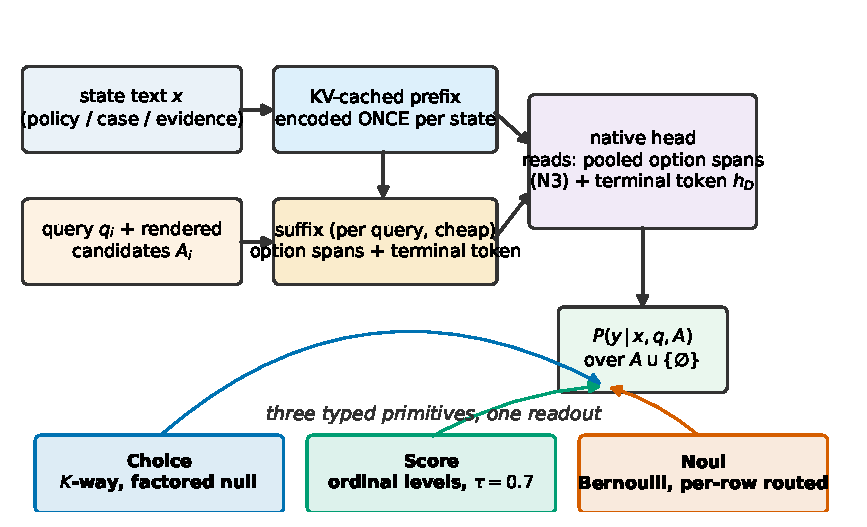
\includegraphics[width=\linewidth]{figures/fig_architecture.pdf}
  \caption{The decision pass. The state is encoded once into a key-value cache. Each question is a short
  causal suffix holding the question and its runtime candidates; the head reads the terminal decision
  state $\hD$ against each candidate's pooled contextual state $\hctx{j}$ at 71\% of backbone depth. One
  readout serves three typed contracts (Choice, Score, Noul), and abstention is a separate gate outside
  the candidate softmax.}
  \label{fig:architecture}
\end{figure}
